\documentclass[aspectratio=169,17pt]{beamer}
\usepackage{booktabs,tikz,helvet}
\usetikzlibrary{positioning,arrows.meta}
\providecommand{\AnalysisPath}{../../results/analysis}
\providecommand{\TracePath}{../../results/visualization}
\input{\AnalysisPath/numbers.tex}
\graphicspath{{\AnalysisPath/}{\TracePath/}}
\setbeamertemplate{navigation symbols}{}
\setbeamertemplate{footline}[frame number]
\setbeamercolor{normal text}{fg=black,bg=white}
\setbeamercolor{frametitle}{fg=black}
\setbeamercolor{title}{fg=black}
\setbeamercolor{structure}{fg=black}
\title{Systolic Array Scaling}
\subtitle{Modeled input supply and complete matrix products}
\author{Ozlem Polat, Thomas Martin, Keith Kamer}
\institute{University of Florida}
\date{}
\begin{document}
\begin{frame}\titlepage\end{frame}

\begin{frame}{Architecture}
\small
\centering
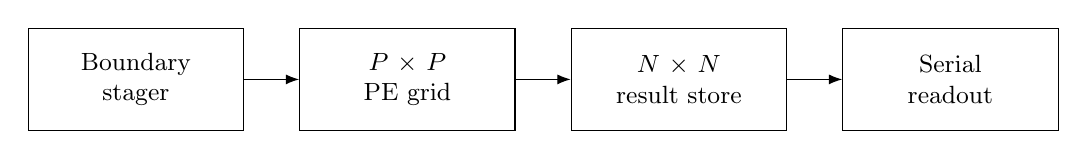
\begin{tikzpicture}[font=\small,>=Latex,box/.style={draw,align=center,text width=25mm,minimum height=13mm}]
\node[box](a){Boundary\\stager};
\node[box,right=7mm of a](b){$P\times P$\\PE grid};
\node[box,right=7mm of b](c){$N\times N$\\result store};
\node[box,right=7mm of c](d){Serial\\readout};
\draw[->](a)--(b);\draw[->](b)--(c);\draw[->](c)--(d);
\end{tikzpicture}
\vspace{5mm}
\begin{itemize}
\item Grids: 2×2, 4×4, 8×8
\item Complete matrix orders: 8 and 16
\item Combined A/B input budgets: 4, 8, 16 words/clock
\item Every output tile streams the full inner dimension
\end{itemize}
\end{frame}

\begin{frame}{Verification evidence}
\small
\begin{itemize}
\item \SimulationCases{} full-width passing cases across \SimulationConfigurations{} configurations
\item Questa sweep and independent GHDL verification agree
\item PE, staging, and synthesis-mode regressions
\item \HardwareConfigurations{} order-16 Vivado implementations
\item Every selected build meets internal setup/hold timing
\end{itemize}
\vspace{1mm}
{\small External I/O delays remain unspecified in the OOC experiment.}
\end{frame}

\begin{frame}{Compute latency}
\centering\includegraphics[width=.96\textwidth,height=.63\textheight,keepaspectratio]{latency_combined.png}\par
\vspace{1mm}
{\footnotesize N=16, full supply: \ComputeLargeTwo{} / \ComputeLargeFour{} / \ComputeLargeEight{} clocks. Largest-grid compute speedup: \WideSpeedup{}×.}
\end{frame}

\begin{frame}{Stalls and structural overhead}
\centering\includegraphics[width=.98\textwidth,height=.62\textheight,keepaspectratio]{cycle_breakdown.png}\par
\vspace{1mm}
{\footnotesize N=16/P=8: restricting supply to four words adds \LimitedStalls{} stalls. Full-supply utilization remains \WideUtilization{}\%.}
\end{frame}

\begin{frame}{Serial readout limits speedup}
\small
\centering
\begin{tabular}{lrr}
\toprule
Full supply, P=8 & N=8 & N=16\\\midrule
Compute clocks & \SmallWideCompute{} & \WideCompute{}\\
Serial readout clocks & \ReadoutSmall{} & \ReadoutLarge{}\\
Total clocks & \SmallWideTotal{} & \WideTotal{}\\
End-to-end speedup & \SmallEndSpeedup{}× & \LargeEndSpeedup{}×\\\bottomrule
\end{tabular}
\vspace{4mm}
\begin{itemize}
\item Readout compresses complete-product speedup
\item 100 MHz rates require successful internal timing
\item GMAC/s calculations exclude external transfers
\end{itemize}
\end{frame}

\begin{frame}{Scaling versus PE count}
\centering\includegraphics[width=.98\textwidth,height=.75\textheight,keepaspectratio]{speedup_full_supply.png}
\end{frame}

\begin{frame}{FPGA resource cost}
\centering\includegraphics[width=.96\textwidth,height=.73\textheight,keepaspectratio]{fpga_resources.png}
\end{frame}

\begin{frame}{Findings and interpretation}
\small
\begin{itemize}
\item Larger grids minimize compute latency in this sweep
\item Smaller grids maximize useful throughput per DSP
\item Input supply and tile overhead limit scaling
\item Result capture/storage affects implementation cost
\item LUT cost peaks at 4×4; DSP count follows PE count
\end{itemize}
\vspace{3mm}
{\small The FPGA comparison uses the three order-16 builds. Simulation covers both matrix sizes. Internal timing is qualified at 100 MHz; board transfers and physical DRAM supply are outside the experiment.}
\end{frame}
\end{document}
